\documentclass{article}


\usepackage{graphicx} % Required for inserting images
\usepackage{amsmath}
\usepackage{amssymb}
\usepackage{bm}
\usepackage{bbm}
\usepackage{color}
\usepackage{url}
\usepackage[export]{adjustbox}

\usepackage{braket}
\title{Spin adapted fermion-to-qubit mappings}

\begin{document}
\section{Unitary Group Approach without the unitary group}
% Standard qubit representations of spin-free fermionic Hamiltonians have redundant degrees of freedom. Any states that differ by a global SU(2) rotation of the spin degrees of freedom will be equivalent under the action of this Hamiltonian. It would be useful if a more compact representation without this degeneracy could be found, as it may enable us to reduce the qubit requirements of our fermion-to-qubit mapping schemes. 
\subsection{UGA}
The Fock space of $2d$-electrons $\bigwedge\mathbb{C}^{2d}$ can be decomposed. As 
\begin{align}
    \bigwedge \mathbb{C}^{d-1}\otimes \mathbb{C}^2 \otimes \bigwedge \mathbb{C}^2 &= \bigwedge \mathbb{C}^{d-1}\otimes \mathbb{C}^2 \oplus \mathbb{C}^2 \\
    &= \bigwedge \mathbb{C}^{d-1}\otimes \mathbb{C}^2 \oplus \mathbb{C}\otimes\mathbb{C}^2\\
    &= \bigwedge (\mathbb{C}^{d-1}\oplus \mathbb{C})\otimes \mathbb{C}^2 \\
    &= \bigwedge \mathbb{C}^{d}\otimes \mathbb{C}^2
\end{align}
Therefore,
\begin{equation}
    \bigwedge\mathbb{C}^{2d}= \bigwedge\mathbb{C}^2 \otimes \bigwedge\mathbb{C}^2 \otimes \cdots \otimes \bigwedge\mathbb{C}^2 = \bigotimes_{d} \bigwedge\mathbb{C}^2
\end{equation}
We can write $\bigwedge \mathbb{C}^2$ in terms of $U(1) \times SU(2)$ irreps as:
\begin{equation}
    \bigwedge \mathbb{C}^2 = 0\otimes 0 \oplus 1 \otimes \frac{1}{2} \oplus 2 \otimes 0
\end{equation}
We perform the repetitive Clebsch-Gordan coupling of these $U(1) \times SU(2)$ irreps to obtain a fully coupled irrep:
\begin{align}
\begin{split}
\label{eq:coupling}
    \bigwedge\mathbb{C}^{2d} &= \bigotimes_{d} \bigwedge\mathbb{C}^2 \\
                            &= \bigotimes_{d} 0\otimes 0 \oplus 1 \otimes \frac{1}{2} \oplus 2 \otimes 0 \\
                            &= \bigoplus_{N,S} W_{N,S}\otimes N\otimes S \\
                            \end{split}
\end{align}
where $W_{N,S}$ is the space of intermediary couplings. 
\subsubsection{Historical Approach (optional)}
At this point we notice that $W_{N,S}$ is equivalent to the $(2^{\frac{N}{2}-S},1^{2S})$ irrep of $U(d)$. We prove this by considering the Gelfand-Tsetlin basis of $U(d)$ which is constructed by recursive restriction of representations from $U(d) \supset U(d-1) \supset \cdots \supset U(1)$. As the restriction $U(i) \supset U(i-1)$ is multiplicity-free and all irreps of $U(1)$ have dimension 1, each path of restrictions uniquely identifies a basis element in the representation of $U(d)$. We can reverse the interpretation and instead think of the Gelfan-Tsetlin basis as a recursive induction of representations that build up to a representation of $U(d)$. Representations of $U(d)$ are labeled by partitions and there are simple rules for finding the possible inductions and Clebsch-Gordan coupling of partitions. 

A induction of irrep $\lambda$ of $U(i)$ to $U(i+1)$ gives a direct sum over all the partitions obtained by adding any number of boxes to $\lambda$ but no two to the same column. Similarly, the Clebsch-Gordan coupling of $\bigwedge\frac{1}{2}$ with irrep $(\lambda_1,\lambda_2)$ of $U(2)$ gives the following:
\begin{align}
    \bigwedge\frac{1}{2}\otimes (\lambda_1,\lambda_2) &= () \otimes (\lambda_1,\lambda_2) \oplus (1) \otimes (\lambda_1,\lambda_2)\oplus (1,1) \otimes (\lambda_1,\lambda_2)\\
    &= (\lambda_1,\lambda_2) \oplus (\lambda_1+1,\lambda_2)\oplus (\lambda_1,\lambda_2+1)\oplus (\lambda_1+1,\lambda_2+1)
\end{align}
Therefore, if we restrict to irreps of $U(i)$ with at most 2 columns then the rules for induction of $U(i) \subset U(i+1)$ and the rules for Clebsch-Gordan coupling of $\bigwedge\frac{1}{2}$ to an irrep of $U(2)$ are conjugate to each other.

Every intermediate coupling $(N,S)$ irrep of $U(1) \times SU(2)$ corresponds to an $(\frac{N}{2}+S,\frac{N}{2}-S)$ irrep of $U(2)$. Therefore, any valid set of intermediary irreps that coupled to $U(2)$ irrep $(\frac{N}{2}+S,\frac{N}{2}-S)$ correspond directly to a valid set of intermediary irreps that induce to $U(d)$ irrep $(2^{\frac{N}{2}-S},1^{2S})$, and hence these intermediary irreps form the Gelfand-Tsetlin basis of $U(d)$ irrep $(2^{\frac{N}{2}-S},1^{2S})$. This correspondence is not simply a coincidence but rather a direct consequence of the Skew Howe duality as we will elaborate on in Appendix A.

Now we have expressed our Hilbert space in terms of representations of the unitary group, we must consider the action of our Hamiltonian on such a space. The ladder operators of $d$-orbital spin-free Hamiltonians ($E_{ij} = \sum_{\mu} a_{i \mu}^{\dagger} a_{j \mu}$) obey the same commutation rules as the generators of $U(d)$. Hence, we can rewrite spin-free Hamiltonians in terms of these generators:
\begin{equation}
    H = \sum_{ij}h_{ij}E_{ij} + \sum_{ijkl}v_{ij,kl}(E_{ik}E_{jl}-\delta_{jk}E_{il})
\end{equation}

The Unitary Group Approach proceeds by finding the matrix elements of the generators of $U(d)$ in the Gelfand-Tsetlin basis of intermediary irreps. Originally this was accomplished by finding matrix elements for local generators (e.g. $\bra{\psi}E_{ii}\ket{\psi'}$,$\bra{\psi}E_{ii+1}\ket{\psi'}$), and then using the recursion relation of the unitary group: $E_{ij+1} =[E_{ij},E_{jj+1}]$. This allowed chemists to work in a smaller Hilbert space by enumerating the possible patterns of intermediary irreps (for a given particle number $N$ and total spin $S$).

However, it is possible to achieve the same results without once resorting to the unitary group! Using the graphical methods of spin algebras numerous independent authors where able to find the matrix elements for the ladder operators in the basis of intermediary irreps. We claim that this approach is effectively a tensor network method, and we restate it using modern notation.
\subsubsection{Modern Approach}
\label{section:modern_approach}
It is possible to graphically represent Eq.~\eqref{eq:coupling} as a fusion tree of $U(1)\times SU(2)$ representations (remembering $\bigwedge \mathbb{C}^2 = 0\otimes 0 \oplus 1 \otimes \frac{1}{2} \oplus 2\otimes 0$):
\begin{figure}[htbp]
    \centering
    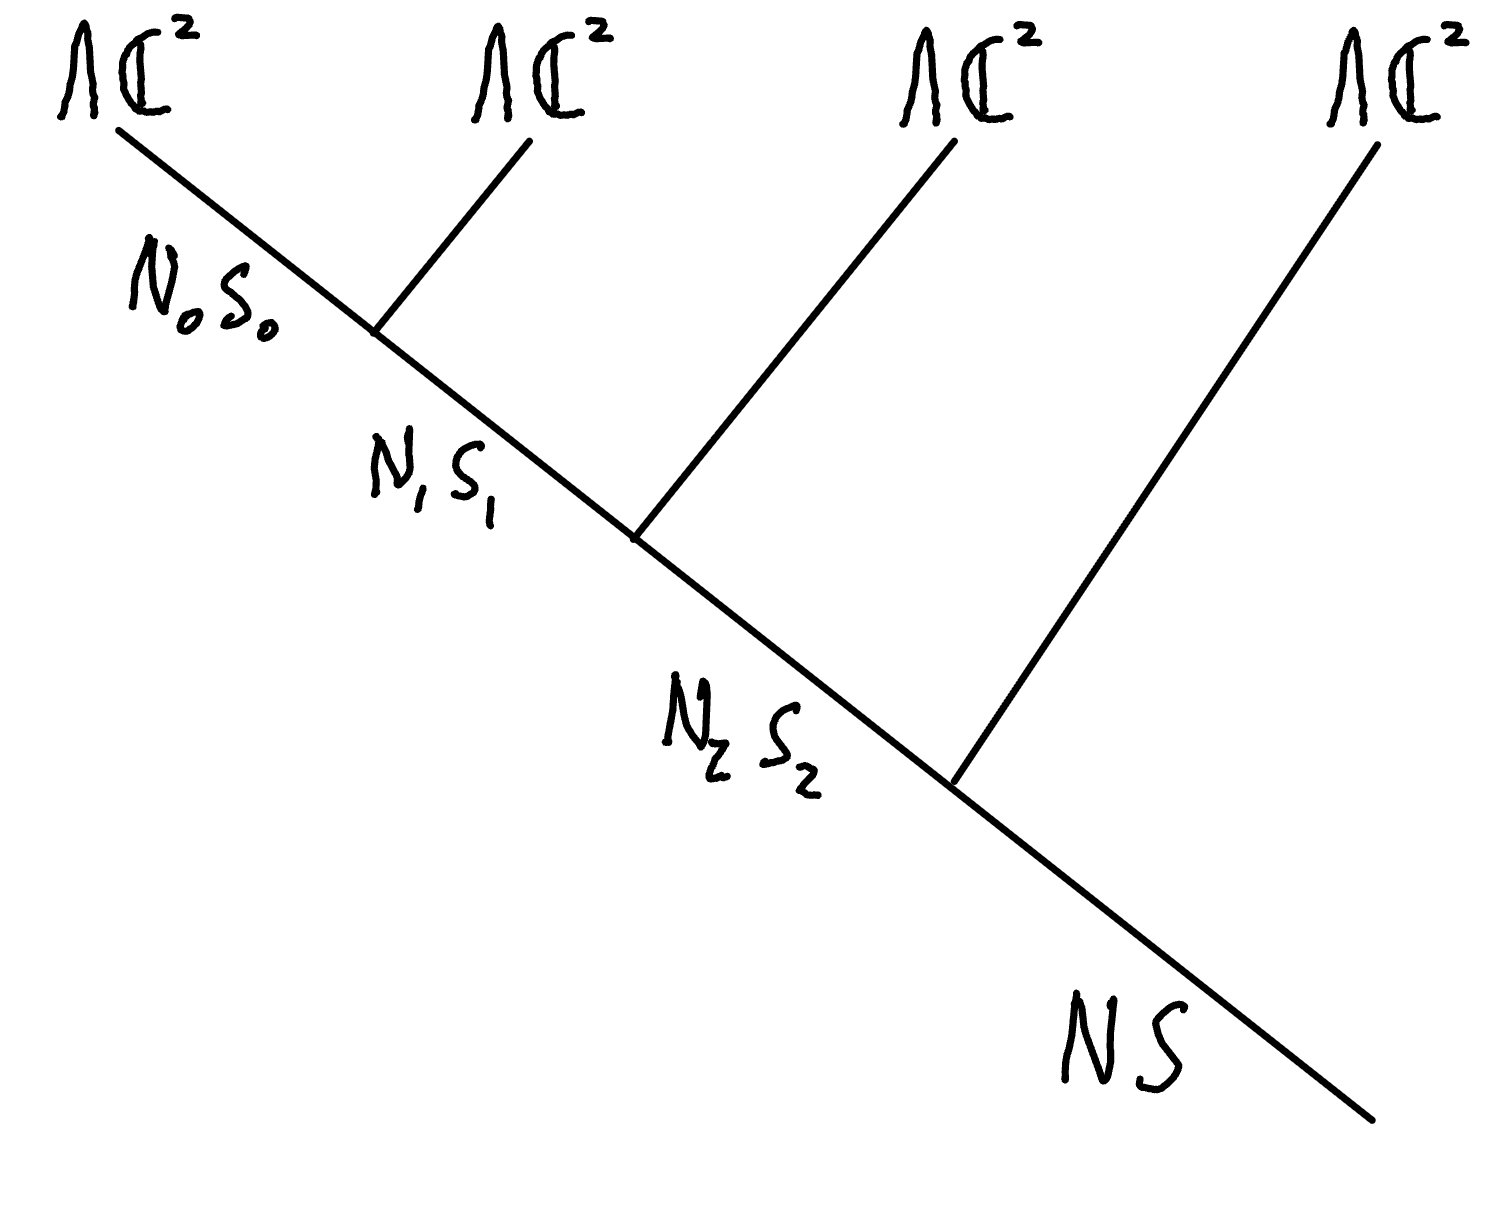
\includegraphics[width=0.5\linewidth]{fusion_tree.png}
    \caption{Caption}
    \label{fig:fusion_tree}
\end{figure}

where $W_{N,S}$ corresponds to the valid choices of $N_0\otimes S_0$, $N_1\otimes S_1$ and $N_2\otimes S_2$ that satisfy this diagram for some $N\otimes S$. 

We can use triple line notation to write Clebsch-Gordan couplings as follows:

\begin{figure}[htbp]
    \centering
    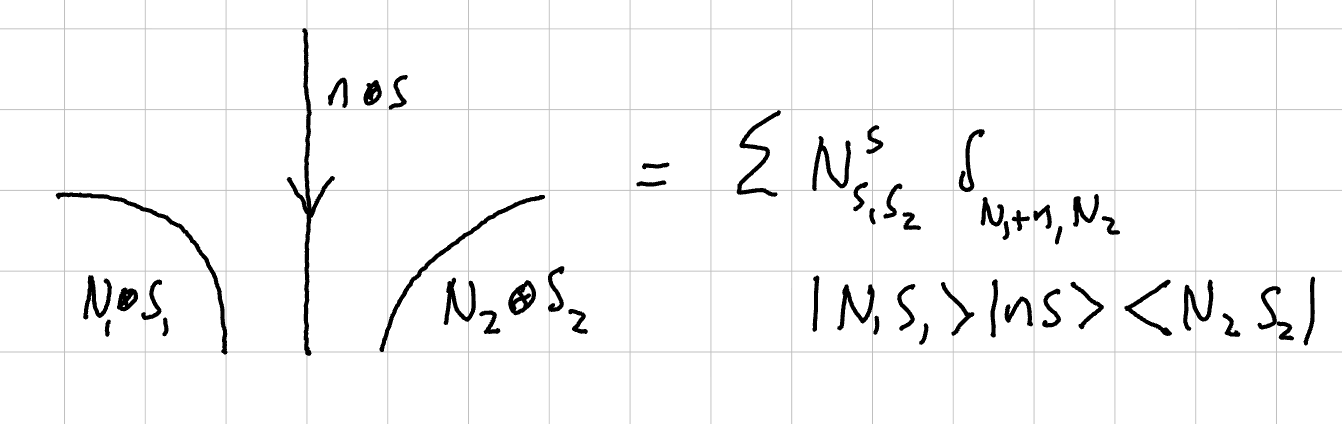
\includegraphics[width=0.5\linewidth]{Clebsch-Gordan.png}
    \caption{Caption}
    \label{fig:placeholder}
\end{figure}
where $S_1 \otimes s = \bigoplus_{S_2} N_{S_1s}^{S_2} S_2$. If a line terminates on its own (rather than as part of a Clebsch-Gordan coupling) then that the end of the line is a representation space corresponding to the label carried by the line. Hence, we can rewrite \eqref{eq:coupling} as an MPO intertwiner:
\begin{figure}[hbtp]
    \centering
    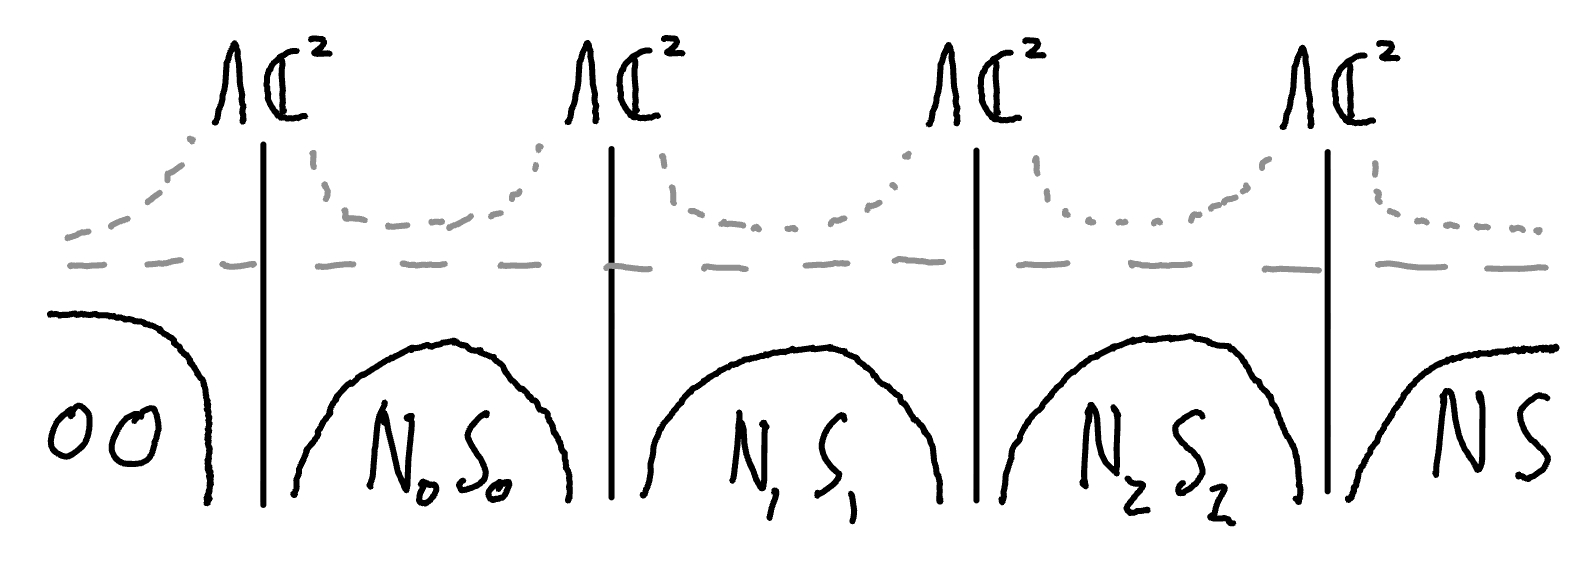
\includegraphics[width=0.5\linewidth]{MPO_duality.png}
    \caption{Caption}
    \label{fig:placeholder}
\end{figure}

This intertwiner represents a duality between the occupation basis and a dual $U(1) \times SU(2)$ basis. We can now use this duality to find an expression for our Hamiltonian terms in the dual basis.

First, we must write down our Hamiltonian term as an MPO in the original theory. It is simple to write down expressions for ladder operators $E_{ab}$ as they directly correspond to a particular choice of bond irrep as can be seen in Fig~\ref{fig:E_ab}.

\begin{figure}[htbp]
    \centering
    $E_{ab}=$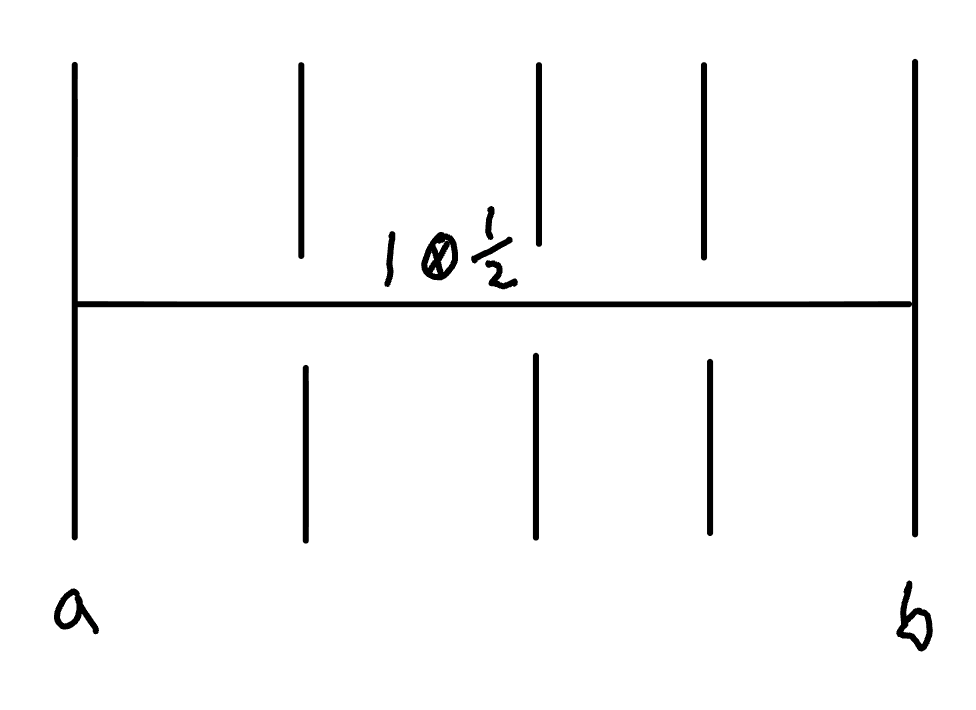
\includegraphics[width=0.5\linewidth, valign=c]{E_ab.png}
    \caption{Caption}
    \label{fig:E_ab}
\end{figure}

We can then find the representation in the dual basis by acting with the duality transformation on both sides of the MPO. Therefore the MPO representation of the operator in the dual theory is given by Fig~\ref{fig:dual_E_ab}.

\begin{figure}[hbtp]
    \centering
    $E_{ab}=$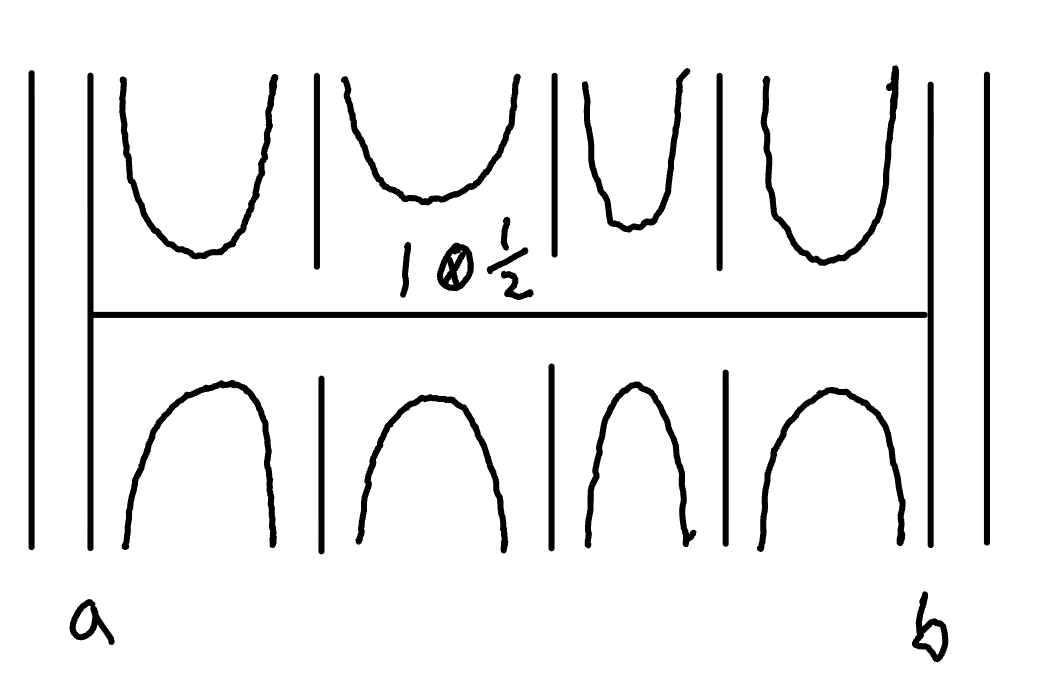
\includegraphics[width=0.5\linewidth, valign=c]{dual_E_ab.png}
    \caption{Caption}
    \label{fig:dual_E_ab}
\end{figure}
We now proceed by factorising this tensor into well known local tensors. To be consistent with other works on generalised dualities we will use F symbols of $SU(2) \times U(1)$ (rather than Wigner-6j symbols) as our local building blocks. However, one can express these F symbols in terms of Wigner-6j symbols:
\begin{multline}
    (F^{(n_1,j_1)(n_2,j_2)(n_3,j_3)}_{(n_4,j_4)})_{(n_5,j_5)}^{(n_6,j_6)} = (-1)^{j_1+j_2+j_3+j_4}\sqrt{2j_5+1}\sqrt{2j_6+1}\begin{pmatrix}
        j_1 &j_2 & j_5\\ j_3&j_4&j_6
    \end{pmatrix} \\\delta_{n_1+n_2,n_5}\delta_{n_3+n_5,n_4}\delta_{n_2+n_3,n_6}\delta_{n_1+n_6,n_4}
\end{multline}
Refs \cite{} show that F symbols can also be expressed by triple line diagrams of the following form:
\begin{figure}[htbp]
    \centering
    \includegraphics[width=0.5\linewidth]{}
    \caption{4 and 3 leg F symbols with arrows going in both directions}
    \label{fig:placeholder}
\end{figure}

The numbers at the termination of each set of triple lines correspond to the order in which the three irreps are fused as it should always go $1 \otimes 2 = 3$. If we wish to contract the 3 legged F symbols with the 4 legged F symbols to get an MPO that resembles our desired form, then we must commute the order of the fusion so they match. To do this we utilise another tensor given by the R symbol which corresponds to a half braiding and can be written in triple line notation as:
\begin{figure}[hbtp]
    \centering
    \includegraphics[width=0.5\linewidth]{}
    \caption{Rsymbol as three lines with different 1,2,3 labels on each end}
    \label{fig:placeholder}
\end{figure}

and has explicit analytic form given by:
\begin{equation}
    R_{(n_3,j_3)}^{(n_1,j_1)(n_2,j_2)} = (-1)^{j_1+j_2-j_3}
\end{equation}
As $R^2=1$ we can factorise our MPO representation of the operator in the dual theory as follows:

\begin{figure}[hbtp]
    \centering
    \includegraphics[width=0.5\linewidth]{}
    \caption{Write out the same diagram as Figure 5 but leave gaps and label by F and R}
    \label{fig:placeholder}
\end{figure}

Now we have a factorised representation of the Hamiltonian term we can proceed with finding matrix elements. By specifying all of the intermediary irreps of $SU(2) \times U(1)$ we uniquely specify the value of every tensor in our factorisation, so we do not need to perform any tensor contraction and instead simply must multiply all the values together. To illustrate this process below we enumerate the possible values of our factorised tensors.
\begin{figure}
    \centering
    \includegraphics[width=0.5\linewidth]{}
    \caption{Factorised tensors}
    \label{fig:placeholder}
\end{figure}
As there are only a small number of ways the intermediary irreps can vary from site to site it is useful to enumerate these using a step vector as shown in the below table:
\begin{table}[htbp]
    \centering
    \begin{tabular}{|c|c|c|}\hline
        $N_{i+1}$ & $S_{i+1}$& $d$ \\
        \hline
        $N_i$ & $S_i$ & 0\\
        $N_i+1$ & $S_i+\frac{1}{2}$ & 1\\
        $N_i+1$ & $S_i-\frac{1}{2}$ & 2\\
        $N_i+2$ & $S_i$ & 3\\\hline
    \end{tabular}
    \caption{Caption}
    \label{tab:placeholder}
\end{table}

Traditional GUGA leverages this by representing each state as paths through a Shavitt graph with the step vector at each site specifying which direction the path chooses. This allows each configuration state function to be stored as a list of step vectors (which has the same storage requirements as the occupation basis). The intermediary irrep labels are stored in the Shavitt graph structure (represented by a distinct row table) and whilst performing the calculation you navigate through this table using the step vectors so you always know the current and next intermediary irrep labels.

For two different paths through the Shavitt graph it is possible to calculate the value of the factorised tensor at site $k$ using the onsite step vectors ($d_k, d'_k$), the $SU(2)$ irrep label of one path ($\frac{b_k}{2}$), and the difference between the $SU(2)$ irrep labels on each path ($\frac{\Delta b_k}{2}$). This is typically done by querying an established table of segment values $W(d_k,d'_k,\Delta b_k,b_k)$, but can now also be calculated on-the-fly using F symbols. For example, for $d_k=0$, $d'_k =2$, $b_k = 2S$, $\Delta b_k = 1$ we have $N_k' = N_k+1$, $N_{k+1}' = N_k +2$, $N_{k+1}=N_k$, $S_k=S$, $S_k' = S+\frac{1}{2}$,$S_{k+1}=S$, $S_{k+1}'=S$, and hence:
\begin{figure}[htbp]
    \centering
    \includegraphics[width=0.5\linewidth]{}
    \caption{3 legged F symbol with the above $N$ and $S$ drawn on and then what this evaluates to}
    \label{fig:placeholder}
\end{figure}

The main advantage of this graphical method over the unitary group method is that it allows for the evaluation of matrix elements for two-electron interactions without summing over all possible intermediary states as was originally done.

\subsection{GUGA with trees}
In Section~\ref{section:modern_approach} we explained how to rewrite GUGA in the language of generalised dualities starting from the fusion tree shown in Fig.~\eqref{fig:fusion_tree}. This is not the unique way to construct a duality between the occupation basis and intermediary irrep labels. One simple modification we could take is instead of working from a fusion tree that sequentially couples each site, we could start from a more complex fusion tree that couples the sites in a tree-like manner. For example,

\begin{figure}[htbp]
    \centering
    \includegraphics[width=0.5\linewidth]{}
    \caption{Tree-like fusion tree}
    \label{fig:placeholder}
\end{figure}

We can follow the same logic as before and express the Hamiltonian terms as MPO operators in this new dual basis:

\begin{figure}[htbp]
    \centering
    \includegraphics[width=0.5\linewidth]{}
    \caption{Operators in tree-like basis}
    \label{fig:placeholder}
\end{figure}

In order to factorise this MPO into local tensors we must introduce a new tensor:

\begin{figure}[htbp]
    \centering
    \includegraphics[width=0.5\linewidth]{}
    \caption{Three legged Clebsch-Gordan fusion tensor (arrows are important)}
    \label{fig:placeholder}
\end{figure}

Now we can proceed to calculate the matrix elements in this dual basis. Under the previous method we needed to calculate the values of all the tensors between $i$ and $j$ as everything outside of this range become a Kronecker delta. In this new method, we only need to calculate the values for the tensors that line on the path through the tree connecting $i$ and $j$ as all the other tensors will reduce to Kronecker deltas. Therefore, by choosing our tree structure to be a full binary tree we can decrease the number of tensors to evaluate for the worst case one-body interaction from $N$ to $O(\log_2N)$ where $N$ is the total number of sites.

\begin{figure}[htbp]
    \centering
    \includegraphics[width=0.5\linewidth]{}
    \caption{Example of computing tree-like factorised matrix element}
    \label{fig:placeholder}
\end{figure}

This new tree-like duality maps to a different dual space and so we will need a new way of enumerating and storing the possible configuration state functions. We can simply store a list the intermediate irrep labels for each configurations state however this can be quite memory intensive. A more compact storage mechanism would be to store the step vectors in a tree data structure. Every site will store a step vector the same as before with only 4 possible values. However, there will be a new step vector at every point the tree branches, the step vector at this point will have $n+1$ possible values where $n$ is the number of ancestors in the shorter of the two branches (as the maximum $SU(2)$ irrep label of the shortest branch will be $\frac{n}{2}$). Therefore for a full binary tree of $N$ sites the storage requirements for the configuration state functions roughly is $3.7N$ bits compared to $2N$ bits required for standard GUGA.

The Shavitt graph description is no longer useful as the sites only have a partial ordering rather than previous linear ordering. Instead we will need a graph of graphs description. Each linear subsection of tree will be described by a collection of Shavitt graphs that run between each possible head and tail intermediary irreps. Then each of these Shavitt graphs will be navigated between by the new branching step vectors which map the head intermediary irreps of two Shavitt graphs to the tail intermediary irrep of the next. Naively this would add additional memory overhead to the algorithm as we must keep track of the position in each active Shavitt graph rather than just one. However, as we only ever need to compute the factorised tensors along a path through the tree we only ever have one Shavitt graph active.

There is a parallel between this and Jordan-Wigner vs tree-like fermion-to-qubit mapping schemes. ...

\subsubsection{Results}

We have implemented this tree-like GUGA and compared it to our implementation of the existing GUGA algorithm. TODO
% \subsection{DMRG}
% Now we understand that GUGA can be thought of as representing our Hamiltonian terms as MPOs in a dual basis, we can use tensor network methods to find the ground state of the Hamiltonian, rather than simply finding matrix elements.

% The first step is to construct a single MPO that represents the full Hamiltonian. In order to do this one must construct a finite state machine MPO that builds all the triple line MPOs needed.

% mention the underlying reason this works is the Howe duality but that this does not generalise as easily as the modern interpretation as it requires every site to have the same single particle representation.

% \subsection{Brief explanation of UGA}
% Unitary Group approach begins with the observation that the ladder operators of $d$-orbital spin-free Hamiltonians ($E_{ij} = \sum_{\mu} a_{i \mu}^{\dagger} a_{j \mu}$) obey the same commutation rules as generators of $U(d)$. Hence, we can rewrite spin-free Hamiltonians in terms of these generators:
% \begin{equation}
%     H = \sum_{ij}h_{ij}E_{ij} + \sum_{ijkl}v_{ij,kl}(E_{ik}E_{jl}-\delta_{jk}E_{il})
% \end{equation}


% \subsubsection{Gelfand-Tsetlin}
% % We do not need to talk about Gelfand-Tsetlin until we have already established which U(d) representations we are considering as this is about choosing the basis for a particular representation
% To use the Hamiltonian in this form we must choose a basis for a representation of $U(d)$. The canonical basis is the Gelfand-Tsetlin basis which is constructed by recursive restriction of representations from $U(d) \supset U(d-1) \supset \cdots \supset U(1)$. As the restriction $U(i) \supset U(i-1)$ is multiplicity-free and all irreps of $U(1)$ have dimension 1, each path of restrictions uniquely identifies a basis element in the representation of $U(d)$. We can reverse the interpretation and instead think of the Gelfan-Tsetlin basis as a recursive inclusion of representations that build up to a representation of $U(d)$. Commonly, Young-Tableus are used to identify the representation of $U(i)$ at each level of inclusion. There is even a set of rules in this language which specifies how the Young-Tableus can be modified under this inclusion. 

% As the representations of $U(d)$ we are considering all have Young-Tabelus with at most 2 columns, it turns out the Young-Tableus rules for inclusion of $U(i) \subset U(i+1)$ are exactly the same as the rules for fusing irreps of $U(2)$ to $()\oplus(1)\oplus(1,1)$. Therefore, we can equivalently specify the Gelfand-Tsetlin basis by the intermediary irreps of $U(2)$ given by fusing $d$ copies of $()\oplus(1)\oplus(1,1)$. Hence the basis of UGA can be rewritten without resorting to the unitary group.
% \begin{equation}
%     E_{ij+1} =[E_{ij},E_{jj+1}]
% \end{equation}
% If we can derive the recursion relation of unitary group operators and the basic weight + nearest neighbour raising and lowering operators without resorting to the unitary group, then the whole of the unitary group approach can be rewritten without reference to the unitary group but rather as the multiplicities of repetitive coupling of irreps of $U(2)$.

% Should discuss in terms of single particle representations

% Crucially the commutation relations of $E_{ij}$ do not imply the anticommutation relations of fermionic operators and can equally arise from bosonic Hamiltonians. Therefore, we only have a valid transformation of our Hamiltonian if we consider it to act on an antisymmetric Hilbert space that reintroduces the anticommutation relations of fermionic operators. The antisymmetric representations of $U(d)$ are given by 1 column Young-Tableus of heights $N \leq d$. The Gelfan-Tsetlin basis of the $\wedge^N \mathbb{C}^d$ representation becomes a list of 1 column Young-Tableus growing by at most 1 box at each inclusion. This can be easily rewritten as a list of which $N$ inclusions added a box. Clearly, this is equivalent to first quantisation, however it is not an accurate representation of a $d$-orbital spin-free Hilbert space which can have up to two electrons per orbital.

% In order to correctly capture the Hilbert space we must include the symmetries of the original Hamiltonian. An $SU(2)$ symmetry is given by $\mathcal{E}_{\mu\nu}= \sum_{i}a_{i\mu}^{\dagger} a_{i\nu}$. The basis for representations of $SU(2)$ is simply given by half-integer $M_S$. Therefore, the Hilbert space must be an antisymmetric 

% The Skew Howe Duality implies that:
% \begin{equation}
%     \bigwedge^N(\mathbb{C}^d\otimes \mathbb{C}^2) = \bigoplus_{\substack{\lambda \vdash N\\l(\lambda
%     ) \leq d\\l(\tilde \lambda
%     ) \leq 2}}\mathbb{S
% }_{\lambda}\mathbb{C}^d\otimes \mathbb{S
% }_{\tilde \lambda}\mathbb{C}^2
% \end{equation}



% \subsubsection{GUGA}

% \subsection{Brief history of Racah algebra techniques}

% \subsection{Unification of GUGA and Racah Algebra as MPOs}

% \subsection{Quantum Paldus Transformation}
% \subsubsection{MPO representation of duality operator}

% \subsection{Operators in the spin-adapted basis}

% \subsubsection{Quantum circuit implementation}

\subsection{Tree-based spin-adapted operators}
One can draw an analogy between the spin-adapted duality we have presented above and the parity fermion-to-qubit mapping. In the parity mapping each qubit stores the parity of the total of occupation numbers of all the fermionic modes below it in the 1D ordering. In our spin-adapted duality each qudit stores the total spin and occupation of all the fermoinic modes below it in the 1D ordering. 

As with the parity mapping we can improve the spin-adapted duality by considering tree based ordering instead. The Bravyi-Kitaev mapping is an example of such an improvement, where each qubit stores the parity of the total occupation numbers of all the fermionic modes that descend from it in the binary tree. For standard fermion-to-qubit mapping schemes this has the effect of shortening the maximum Pauli weight of a fermionic operator from $O(N)$ to $O(\log N)$.

We can repeat this improvement for the spin-adapted duality by performing the Clebsch-Gordan couplings in a tree-like fashion rather than in a linear order. This gives us a new tree-like spin-adapted duality which allows one to represent symmetric operators with MPOs with maximum $O(\log N)$ sites compared to the previous $O(N)$ sites. Hence, using this approach we are able to exponentially reduce the cost of computing the matrix elements for long-range interactions in the dual basis.

This has far ranging implications for all of the applications we previously discussed. Not only does it represent a significant step forwards in two previously separate areas of long established research: GUGA and Racah Algebra, but it also provides a framework for implementing efficent quantum circuits for spin-adapted operators on a quantum computer.

% \subsection{Local spin-adapted operators}
% It is possible to go one step further in drawing inspiration from fermion-to-qubit mappings and implement local spin-adapted duality...


% Block2 is state of the art for dmrg on quantum chemistry and has best method for constructing hamiltonian mpo
\end{document}